% !TEX program = xelatex
% Compile: xelatex squeezing_paper.tex (run twice for references).
% English-only source; also compiles with pdflatex.
% Figures: docs/squeezing_report/paper_figs/ (built by make_paper_figs.py).
\documentclass[11pt,a4paper]{article}

\usepackage[T1]{fontenc}
\usepackage{amsmath,amssymb}
\usepackage{graphicx}
\usepackage{booktabs}
\usepackage{array}
\usepackage{tabularx}
\usepackage{geometry}
\geometry{margin=2.4cm}
\usepackage{caption}
\captionsetup{font=small,labelfont=bf}
\usepackage{enumitem}
\usepackage{xcolor}
\usepackage[hidelinks]{hyperref}
\graphicspath{{paper_figs/}}
\sloppy

\newcommand{\dB}{\,\mathrm{dB}}
\newcommand{\GHz}{\,\mathrm{GHz}}
\newcommand{\MHz}{\,\mathrm{MHz}}
\newcommand{\degC}{\,^{\circ}\mathrm{C}}
\newcommand{\Rb}{$^{85}$Rb}

\title{\textbf{Locating and hardening the operating point of\\
intensity-difference squeezing from four-wave mixing in hot $^{85}$Rb:\\
a simulation case study}}
\author{Suin Park}
\date{July 8, 2026}

\begin{document}
\maketitle

\begin{abstract}
\noindent
We report a systematic numerical study of twin-beam intensity-difference
squeezing (IDS) generated by double-$\Lambda$ four-wave mixing (FWM) on the
\Rb{} D1 line, carried out with an internal steady-state Floquet--Maxwell--Bloch
simulation whose full source code is publicly available.
Anchoring all fixed parameters to a recent single-laser FWM experiment
[Sim \emph{et al.}, Sci.\ Rep.\ \textbf{15}, 7727 (2025)], we scan the
squeezing over the pump one-photon detuning $\Delta$ and the cell temperature
$T$, with the two-photon detuning $\delta$ optimized at each point. The final
model predicts a recommended operating point at
$\Delta=-1.50\GHz$ (relative to $F{=}2\to F'{=}3$), $T=110\degC$,
$\delta=-280\MHz$, where the simulated squeezing reaches $\xi=-8.10\dB$ at a
realistic detection efficiency $\eta=0.869$ --- within $0.7\dB$ of the
detection floor $10\log_{10}(1-\eta)=-8.84\dB$, and $0.32\dB$ deeper than the
best blue-detuned operating point near the conventional experimental choice. A
five-parameter tolerance analysis around this point yields, for a
$+0.5\dB$ degradation budget, allowed drifts of $+2.1$ percentage points in
detection-path loss, $-9.6/{+}4.2\MHz$ in two-photon detuning,
$-32/{+}155\MHz$ in one-photon detuning, and $-3.3/{+}12\degC$ in cell
temperature, with no measurable sensitivity to seed power between 1 and
64\,$\mu$W; the resulting troubleshooting priority is
loss $\to$ two-photon detuning $\to$ one-photon detuning $\to$ temperature
$\to$ seed power.

We deliberately present the study as a chronological case study, because
three successive, superficially plausible results produced along the way
turned out to be spurious: a broad ``maximum'' that was in fact a
detection-floor degeneracy, making the naive question ``where is the
maximum?'' ill-posed; a $-82\dB$ prediction traced to a catastrophically
canceling noise formula with the wrong high-gain asymptote; and an
extreme-gain optimum created by an objective function blind to the
absorption that generates the gain. Each defect was
caught by an internal-consistency guardrail (a detection-floor bound, a
twin-beam gain-gap criterion, cross-evaluation of independent formulas on
identical gain data, and a sign audit of the sideband beat), and we distill
these guardrails into a checklist for simulation-based predictions of
squeezing experiments.
\end{abstract}

\tableofcontents
\bigskip

%==================================================================
\section{Introduction}
%==================================================================
Non-degenerate four-wave mixing in hot alkali vapor converts two pump photons
into a probe (signal) photon and a conjugate photon. Because the photons are
created strictly in pairs, the intensities of the two output beams are so
strongly correlated that the noise of their difference $N_s-N_c$ falls below
the shot-noise limit, producing \emph{intensity-difference squeezing} that
can be observed with direct balanced detection --- no local oscillator
required. Since the first strong
demonstrations in rubidium vapor \cite{McCormick2007,Pooser2009}, the
double-$\Lambda$ scheme on the \Rb{} D1 line has become a workhorse source of
bright twin beams, with measured squeezing of $-8\dB$ and beyond, and it
remains under active development, including single-diode-laser
implementations \cite{Sim2025} and long-term-stabilized operation
\cite{Allen2026}. It is also well established experimentally that the
best squeezing is \emph{not} obtained at the highest gain: absorption and
loss compete with the parametric process, so the optimum operating point is
set by a trade-off \cite{Jasperse2011}.

For an experimentalist setting up such a source, the practical questions are
concrete. Where in the plane of pump one-photon detuning $\Delta$ and cell
temperature $T$ (equivalently, atomic density) is the squeezing deepest? What
physically limits the attainable depth? And how tightly must each knob ---
detunings, temperature, seed power, detection loss --- be controlled before
the squeezing degrades noticeably? This paper answers these questions with a
first-principles steady-state simulation of the double-$\Lambda$ system,
calibrated once against the reference experiment of Sim \emph{et al.}
\cite{Sim2025} and then used to scan the full operating plane. All
computations were performed with an internal simulation code; the complete
source, the archived scan data, and the scripts that regenerate every figure
in this paper are publicly available on GitHub \cite{repo}.

We have chosen to present the study \emph{chronologically}, as a case study
in five stages, rather than presenting only the final model. The reason is
methodological honesty: along the way the simulation produced three
successive answers that looked plausible and were later shown to be wrong ---
one conceptually ill-posed question, one outright formula bug amplified by
floating-point cancellation, and one artifact of an objective function that
did not charge the physical cost of the gain it rewarded. Each wrong answer
survived until a specific internal-consistency check exposed it. We believe
the sequence of failures and the guardrails that caught them are at least as
useful to the community as the final numbers, because the same failure modes
threaten any simulation-based optimization of a squeezing experiment. Readers
interested only in the final predictions can skip to
Secs.~\ref{sec:stage5}--\ref{sec:tolerance}; the guardrail checklist is
collected in Sec.~\ref{sec:discussion}.

%==================================================================
\section{The simulation}
\label{sec:model}
%==================================================================

\subsection{Physical model}
The atomic system is the standard double-$\Lambda$ configuration on the \Rb{}
D1 line: the two hyperfine ground states $F=2,3$ (splitting
$\nu_{\mathrm{HF}}=3.035732439\GHz$) and the two excited states $F'=2,3$. A
strong pump of power $P_{\mathrm{pump}}$ drives both legs; a weak seed
(probe) is injected on the $(-)$ Raman branch and a conjugate builds up on
the opposite sideband. Rabi frequencies follow from the beam intensities,
$I=2P/(\pi w_0^2)$ and $\Omega=\Gamma\sqrt{I/(2I_{\mathrm{sat}})}$, with the
measured beam waists.

For each probe frequency and each atomic velocity class the simulation
solves the steady state of the driven system in a Floquet sideband expansion
and extracts the dimensionless susceptibility matrix
$(\bar\chi_{ss},\bar\chi_{sc},\bar\chi_{cs},\bar\chi_{cc})$ that couples the
probe and conjugate fields. After Doppler averaging over the Maxwell
velocity distribution, the two sidebands are propagated through the cell
with the linearized coupled-mode equation
\begin{equation}
\frac{d}{dz}\begin{pmatrix}\Omega_s\\ \Omega_c^{*}\end{pmatrix}
= M\begin{pmatrix}\Omega_s\\ \Omega_c^{*}\end{pmatrix},
\qquad
G_s=\bigl|\mathcal{T}_{00}\bigr|^2,\quad G_c=\bigl|\mathcal{T}_{10}\bigr|^2,
\label{eq:prop}
\end{equation}
where $\mathcal{T}=\exp(ML)$ is the transfer matrix of the cell of length
$L$ and $G_s$, $G_c$ are the probe and conjugate power gains. The
propagation is segmented along the cell, with the pump power depleted
self-consistently segment by segment (energy conservation caps the total
gain at $G_{\mathrm{cap}}=1+P_{\mathrm{pump}}/(2P_{\mathrm{seed}})$), and
includes an iteratively converged longitudinal phase mismatch $\Delta k_z$, the
Gaussian overlap of the pump and probe modes at their crossing angle
$\theta$, and Clebsch--Gordan-weighted effective couplings that fold in the
Zeeman substructure (a full Zeeman-resolved Floquet solve is deferred).
The atomic density follows from the cell temperature through the
vapor-pressure curve. Density- and temperature-dependent collisional
decoherence is included both for the optical coherences (resonant
self-broadening, $\Gamma_{\mathrm{eff}}=\Gamma+\beta N$) and for the
ground-state Raman coherence (transit-time floor plus Rb--Rb collisions).

\subsection{From gains to measured squeezing}
\label{sec:noisemodel}
For a lossless twin-beam source the photon-number difference is a conserved
quantity of the parametric interaction, which fixes the intensity-difference
noise (normalized so that $S=1$ is the shot-noise limit) to
\begin{equation}
S_{\mathrm{src}}=\frac{(G_s-G_c)^2}{G_s+G_c}
\;\xrightarrow[\;G_c=G_s-1\;]{}\;\frac{1}{2G_s-1}.
\label{eq:sideal}
\end{equation}
The high-gain behavior $S\propto 1/(2G)$ matches the standard result of the
experimental literature \cite{Sim2025}; an earlier, incorrect version of
this formula plays a central role in Sec.~\ref{sec:stage3}.

Losses are applied as beam splitters in three tiers. Inside the cell each
sideband is attenuated by its own linear absorption: the probe and the
conjugate sit at different optical frequencies
($f_c = 2\Delta - f_{\mathrm{probe}}$ in the rotating frame of the pump) and
each samples the $F{=}2\to F'$ absorption manifold at its own frequency,
giving arm transmissions $\tau_{s,c}=e^{-\mathrm{OD}_{s,c}}$. The
parametric susceptibilities of the four-level model do not contain this
linear absorption of the full hyperfine manifold, so it is computed from a
separately validated absorption model (verified to $<0.1\%$ against
laboratory optical-depth data) and imposed on each arm without any adjustable
coefficient. A small amount of pump light scattered into the detection modes
is modeled as an incoherent noise contribution anchored to the (validated)
pump optical depth, $\propto\kappa\,(1-e^{-\mathrm{OD}_{\mathrm{pump}}})$,
with $\kappa=0.1$ the only residual coefficient of this \emph{extended
excess-noise model}; the results below are insensitive to $\kappa$ (the
artifact suppression reported in Stage IV persists even at $\kappa=0$).
Unequal arm losses are combined in a standard balanced-detector noise model
for two partially correlated beams. Finally, the total detection efficiency
$\eta=\mathrm{QE}\,(1-\ell)$, with $\ell$ the post-cell optical loss, acts
symmetrically on both arms:
\begin{equation}
S(\eta)=\eta\,S_{\mathrm{cell}}+(1-\eta),
\qquad
\xi=10\log_{10}S(\eta)\;[\mathrm{dB}].
\label{eq:eta}
\end{equation}
Because $S_{\mathrm{cell}}\ge 0$, Eq.~\eqref{eq:eta} implies the
\emph{detection floor}
\begin{equation}
\boxed{\;\xi \ \ge\ \xi_{\mathrm{floor}}=10\log_{10}(1-\eta)\;}
\label{eq:floor}
\end{equation}
for every operating point: no simulated (or measured) squeezing can be
deeper than the vacuum noise admitted by the detection loss. Equation
\eqref{eq:floor} requires only $S_{\mathrm{cell}}\ge 0$ and is therefore
independent of any modeling error upstream --- which is precisely what makes
it useful as a guardrail (Sec.~\ref{sec:stage1}).

Two properties of this chain are worth noting. First, $\eta$ is pure
post-processing: the gains and in-cell losses do not depend on it, so a
single scan of the $(\Delta,T)$ grid can be re-read at any detection
efficiency essentially for free. Second, loss can only move $S$ \emph{toward}
shot noise; it can never push the difference noise above it. Observed
anti-squeezing (positive dB) therefore always signals excess noise ---
pump-noise coupling, spontaneous Raman scattering, or leakage of the large
anti-squeezed intensity-\emph{sum} noise through detector imbalance --- and
never mere attenuation.

\subsection{Conventions}
\label{sec:conventions}
Throughout the paper, the one-photon detuning $\Delta$ is the pump detuning
from the \Rb{} D1 $F{=}2\to F'{=}3$ transition,
$\omega_{\mathrm{pump}}=\omega(F{=}2\to F'{=}3)+\Delta$, matching the
convention of Ref.~\cite{Sim2025}. The two-photon detuning $\delta$ is
defined through the seed frequency on the $(-)$ Raman branch,
\begin{equation}
\omega_{\mathrm{seed}}=\omega_{\mathrm{pump}}-\nu_{\mathrm{HF}}+\delta ,
\label{eq:tpd}
\end{equation}
so that the physical pump--seed beat note is $\nu_{\mathrm{HF}}-\delta$ (the
sign convention in Eq.~\eqref{eq:tpd} is the subject of the audit in
Sec.~\ref{sec:stage5}). The pump--probe crossing angle is
$\theta=0.32^{\circ}$, the geometry of the reference experiment, unless
stated otherwise. The measured squeezing $\xi$ is always reported in dB,
with negative values meaning noise below the shot-noise limit.

\subsection{Calibration and reference parameters}
All parameters other than the scanned variables are pinned to the reference
experiment \cite{Sim2025} and are listed in Table~\ref{tab:ref}. The
line-strength scale of the propagation is fixed by physical coupling
normalization plus one residual calibration factor anchored at the reference
operating point; this factor was \emph{not} re-tuned after any of the model
revisions described below. With $\mathrm{QE}=0.92$ and post-cell loss
$\ell=5.5\%$, the reference detection efficiency is $\eta=0.8694$ and the
detection floor is $-8.8406\dB$.

\begin{table}[ht]
\centering
\caption{Reference parameters (fixed in all scans unless stated otherwise).}
\label{tab:ref}
\begin{tabular}{lll}
\toprule
Quantity & Value & Note\\
\midrule
Pump power $P_{\mathrm{pump}}$ & $600$\,mW & Ref.~\cite{Sim2025}\\
Seed power $P_{\mathrm{seed}}$ & $8\,\mu$W & Ref.~\cite{Sim2025}\\
Cell length $L$ & $12.5$\,mm & \\
Pump / seed waists & $530$ / $330\,\mu$m & \\
Pump--probe angle $\theta$ & $0.32^{\circ}$ & default geometry\\
Raman branch & $(-)$ & standard seeded readout\\
Detector quantum efficiency & $0.92$ & recalibrated in Stage II\\
Post-cell optical loss $\ell$ & $5.5\%$ & \\
\midrule
$\eta=\mathrm{QE}(1-\ell)$ & $0.8694$ & \\
Detection floor $10\log_{10}(1-\eta)$ & $-8.8406\dB$ & Eq.~\eqref{eq:floor}\\
\bottomrule
\end{tabular}
\end{table}

\subsection{The five stages at a glance}
Table~\ref{tab:stages} summarizes how the model and the conclusions evolved.
Each stage is described in its own section below. Only the Stage-V numbers
are quantitatively current; every earlier coordinate or depth quoted in this
paper is explicitly historical and is accompanied by the reason it was
superseded.

\begin{table}[ht]
\centering
\caption{Chronology of the study. Each stage's scan was run with the model
content accumulated up to that row.}
\label{tab:stages}
\small
\begin{tabularx}{\textwidth}{l>{\raggedright\arraybackslash}X>{\raggedright\arraybackslash}X}
\toprule
Stage & Model content added & Outcome / defect exposed\\
\midrule
I (\S\ref{sec:stage1}) & lossless parametric source + detection efficiency &
``maximum squeezing'' is ill-posed: everything collapses onto the detection
floor; objective reframed as an \emph{efficient-frontier} search\\
II (\S\ref{sec:stage2}) & full propagation: in-cell probe absorption,
segmented pump depletion, phase mismatch, Gaussian overlap, CG-weighted
Zeeman corrections; detection efficiency recalibrated &
in-cell loss creates a genuine interior optimum in $T$; transparency window
identified\\
III (\S\ref{sec:stage3}) & wide ideal-detection scan; then corrected
difference-noise formula, collisional decoherence, twin-beam gap gate &
spurious $-82\dB$ traced to a formula bug (catastrophic cancellation, wrong
asymptote)\\
IV (\S\ref{sec:stage4}) & per-sideband linear absorption + pump scatter
(``extended excess-noise model'') &
extreme-gain artifact removed ($G_s\,636\to 27$); red/blue lobe
near-degeneracy identified\\
V (\S\ref{sec:stage5}) & sideband-beat sign correction &
optimum relocates to $(-1.50\GHz,\,110\degC)$; final frontier, ideal limit,
geometry study, tolerance analysis\\
\bottomrule
\end{tabularx}
\end{table}

%==================================================================
\section{Stage I: the ill-posed maximum}
\label{sec:stage1}
%==================================================================
The study began with the most obvious question: fix everything at the
reference values and find the $(\Delta,T)$ that gives the deepest squeezing.
The first scan (684 grid points, $\Delta\in[-0.5,3.0]\GHz$,
$T\in[60,150]\degC$, with $\delta$ optimized at each point) used the
simplest defensible model: a lossless parametric source characterized by
$(G_s,G_c)$, followed by the detection efficiency of Eq.~\eqref{eq:eta}. At
this stage the efficiency was calibrated at $\eta=0.855$, giving a floor of
$-8.385\dB$. (The detector
quantum efficiency was recalibrated from $0.905$ to $0.92$ in Stage II,
moving the floor to $-8.841\dB$; the Stage-I numbers quoted here are
historical.)

The result was unambiguous and, at first sight, disappointing: the deepest
squeezing found anywhere on the grid was $-8.385\dB$ --- the detection floor
itself, reproduced to four decimal places --- and \emph{no} grid point fell
below the floor ($0/684$). More than a quarter of the grid sat within
$0.01\dB$ of the floor. The ``maximum'' was not a point but a broad plateau
(Fig.~\ref{fig:stage1plateau}).

The mechanism is elementary and worth stating precisely, because it recurs
throughout the paper (Fig.~\ref{fig:floor}). For balanced twin beams the
source noise falls off with gain --- in the corrected formula of
Eq.~\eqref{eq:sideal} as $S_{\mathrm{src}}\simeq 1/(2G_s)$ --- so beyond a
modest ``knee'' ($G_s\gtrsim 30$ at the reference efficiency) the term
$\eta\,S_{\mathrm{src}}$ becomes negligible compared with the vacuum leakage
$(1-\eta)$, and
\begin{equation}
S(\eta)\;\longrightarrow\;1-\eta .
\end{equation}
Gain is exponential in atomic density and hence double-exponential in
temperature, so the knee is crossed almost everywhere at high temperature,
and a large two-dimensional region maps onto one and the same number. Two
consequences follow:

\begin{enumerate}[nosep]
\item \textbf{The question ``where is the maximum?'' is ill-posed} at finite
      detection efficiency. The answer is a degenerate plateau whose height
      is a property of the \emph{detector}, not of the atoms. The only
      meaningful optimization is the \emph{efficient frontier}: the operating
      point that reaches the floor at the lowest cost in temperature, gain,
      and optical depth --- quantities that also control the excess-noise
      channels (pump scatter, collisional dephasing, anti-squeezed sum-noise
      leakage) that a static model does not capture.
\item \textbf{The floor is a guardrail.} Equation~\eqref{eq:floor} holds for
      \emph{any} physical source, however elaborate the propagation model.
      Any simulated point deeper than $10\log_{10}(1-\eta)$ is a numerical or
      coding error by construction. This check is applied to every scan in
      this paper; its underlying spirit --- distrust any implausibly deep
      value --- is also what eventually exposed the Stage-III bug, in a scan
      where the floor itself had been removed.
\end{enumerate}

The gain lever and the efficiency lever separate cleanly: at fixed
$\eta=0.855$, raising $G_s$ from 10 to 300 improves $\xi$ by less than
$0.2\dB$, whereas at fixed high gain, raising $\eta$ from $0.855$ to $0.95$
deepens the floor from $-8.4$ to $-13.0\dB$. In this class of experiments
the squeezing depth is bought at the detector, not in the vapor cell.

\begin{figure}[ht]
\centering
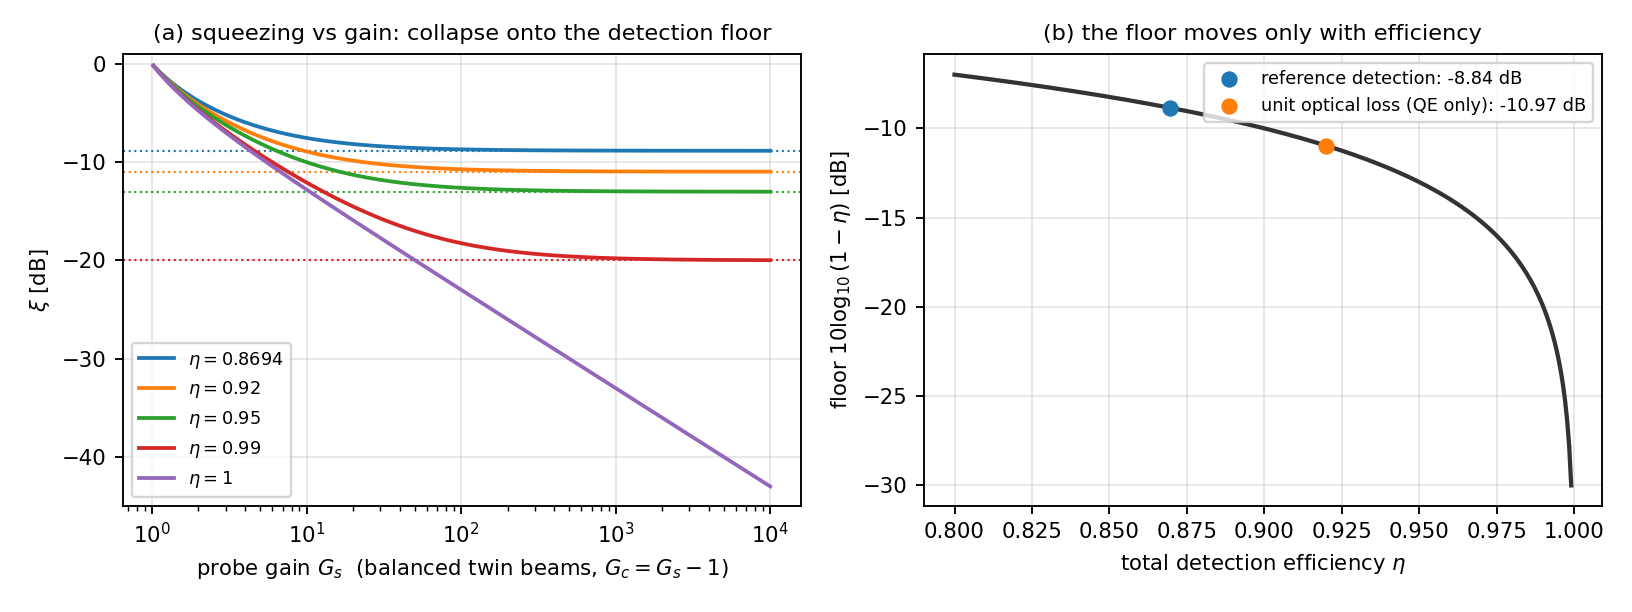
\includegraphics[width=\textwidth]{fig1_floor_theorem.png}
\caption{The detection-floor mechanism (analytic, using
Eqs.~\eqref{eq:sideal}--\eqref{eq:eta} with balanced twin beams).
(a)~Squeezing versus probe gain for several detection efficiencies: each
finite-$\eta$ curve saturates at its floor $10\log_{10}(1-\eta)$ (dotted),
and only $\eta=1$ improves indefinitely. The marginal value of gain is
essentially exhausted by $G_s\approx 30$. (b)~The floor as a function of
$\eta$; the two markers correspond to the recalibrated reference detection
($\eta=0.8694$) and to a hypothetical lossless setup limited only by the
detector quantum efficiency ($\eta=0.92$).}
\label{fig:floor}
\end{figure}

\begin{figure}[ht]
\centering
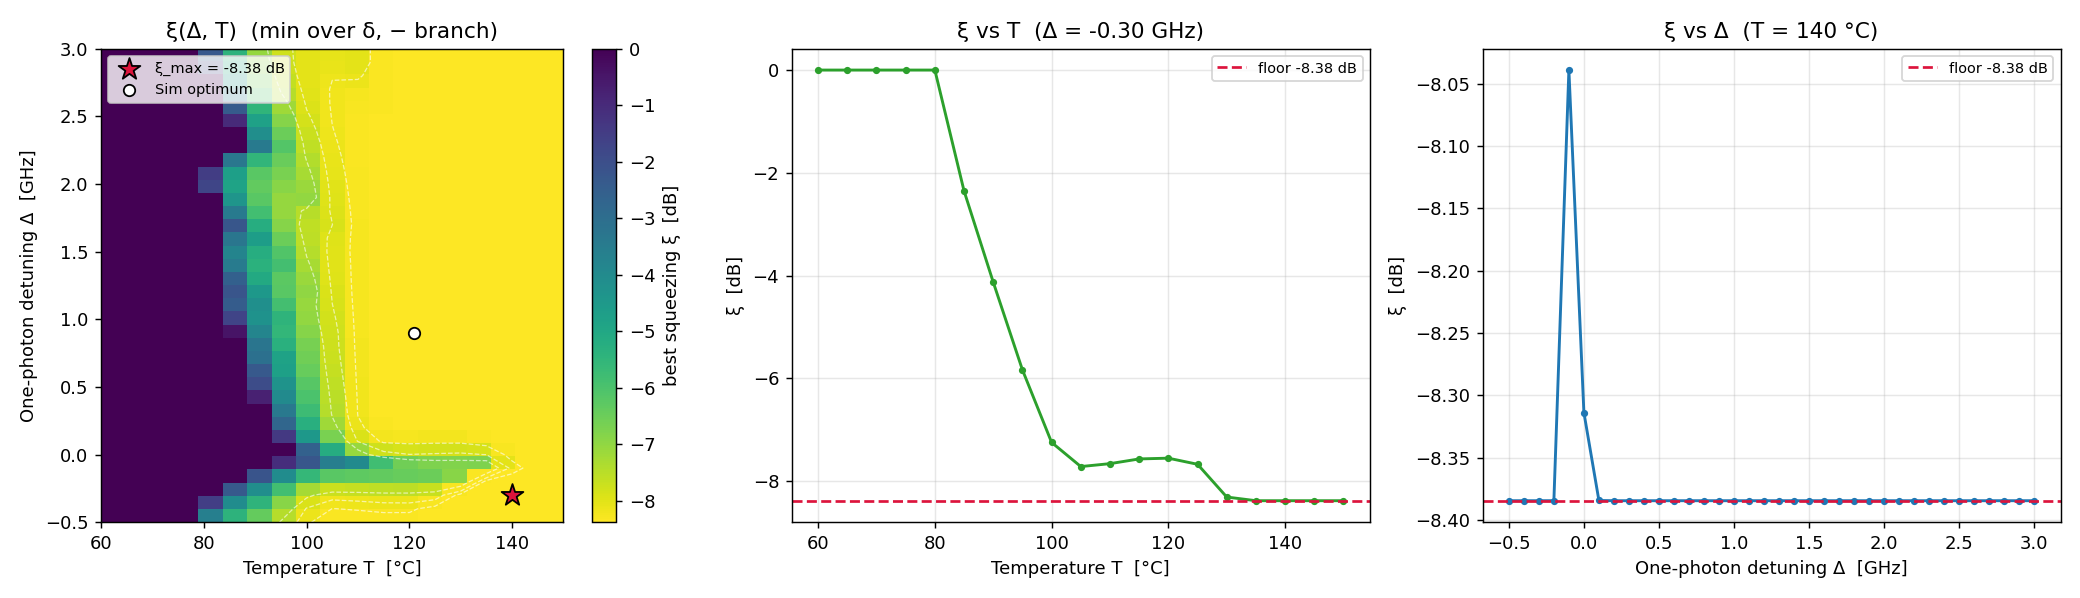
\includegraphics[width=\textwidth]{fig2_stage1_plateau.png}
\caption{Archived Stage-I scan (shown as produced at that stage; the
original scan archive was later overwritten, so the figure is reproduced
from the archived image). Left: $\xi(\Delta,T)$ with the low-temperature
no-gain region ($\xi=0$) giving way to the floor plateau at high
temperature. Middle: temperature dependence at the optimal detuning ---
monotonic asymptotic approach to the floor. Right: detuning dependence at
fixed $T$. Computed with the Stage-I model (pre-correction noise formula,
no in-cell loss) and the Stage-I efficiency calibration ($\eta=0.855$,
floor $-8.385\dB$); the plateau phenomenology, though not the numbers,
survives all later model revisions.}
\label{fig:stage1plateau}
\end{figure}

%==================================================================
\section{Stage II: in-cell loss creates a real interior optimum}
\label{sec:stage2}
%==================================================================
The Stage-I model treated the vapor as a pure gain medium. In reality the
twin beams propagate through an optically thick resonant vapor, and the
absorption they suffer \emph{inside} the cell is not part of the detection
efficiency --- it depends on $(\Delta,T)$ and grows steeply with density.
Stage II therefore upgraded the propagation to the full model of
Sec.~\ref{sec:model} (segmented pump depletion, self-consistent phase
mismatch, Gaussian overlap, CG-weighted Zeeman corrections) and, crucially,
added the
in-cell optical depth of the probe as a distributed loss,
$S_{\mathrm{cell}}=\tau S_{\mathrm{src}}+(1-\tau)$ with
$\tau=e^{-\mathrm{OD}}$. The detector quantum efficiency was simultaneously
recalibrated to $0.92$ against the reference experiment's detection budget,
setting the floor at $-8.8406\dB$, its final value.

This changed the phenomenology in one essential way: at detunings where the
vapor absorbs, $\xi(T)$ is no longer monotonic. Low temperature starves the
gain; high temperature multiplies the optical depth; and in between a
genuine interior optimum appears. A map of the in-cell optical depth shows
an absorption wedge opening around $\Delta\in[-1.2,+0.5]\GHz$ for
$T\gtrsim 90\degC$, flanked by transparency: detunings a few GHz to the red
of the $F{=}2\to F'{=}3$ line stay optically thin up to high temperature
(Fig.~\ref{fig:stage2od}).

As computed at this stage, the global optimum sat in the transparency window
($\Delta=-2.2\GHz$, $T=140\degC$) exactly on the recalibrated floor, and the
cheapest operating point reaching within $0.1\dB$ of it was at
$\Delta\approx-1.9\GHz$, $T\approx120\degC$ with a moderate gain
$G_s\approx 32$; a fixed readout at the reference experiment's detuning
($+0.9\GHz$, $120\degC$) gave $-7.9\dB$, consistent in magnitude with the
measured $-7.8\dB$ of Ref.~\cite{Sim2025}. These specific coordinates did
not survive the later corrections (Secs.~\ref{sec:stage3}--\ref{sec:stage5})
and are quoted only to document the trajectory of the study. What did
survive was the structural conclusion: \emph{in-cell absorption converts the
degenerate plateau into a real optimization problem}, with a
temperature-detuning trade-off of exactly the kind long emphasized in the
experimental literature \cite{Jasperse2011}.

\begin{figure}[ht]
\centering
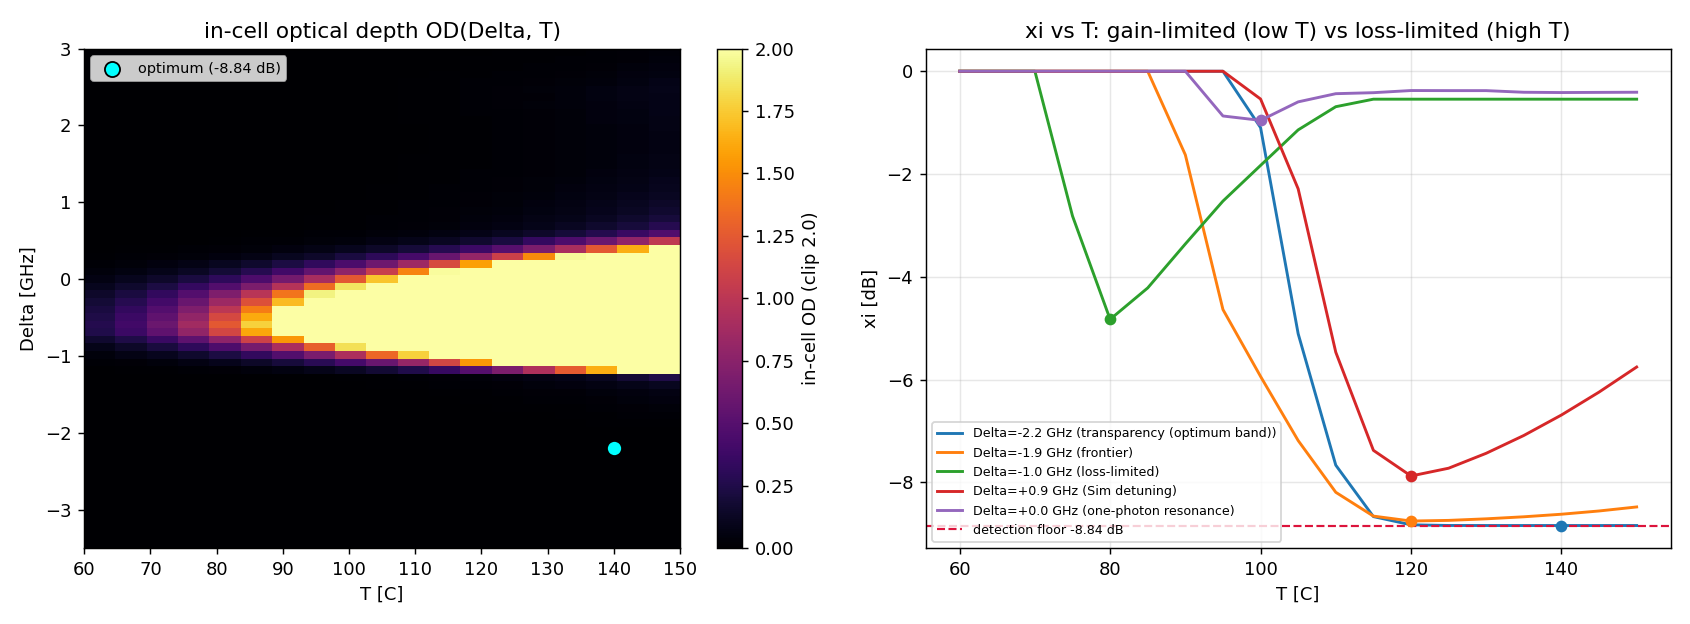
\includegraphics[width=\textwidth]{fig3_stage2_od.png}
\caption{Archived Stage-II diagnostic (shown as produced at that stage; the
original scan archive was later overwritten). Left: in-cell optical depth
$\mathrm{OD}(\Delta,T)$, showing the absorption wedge around
$\Delta\in[-1.2,+0.5]\GHz$ opening with temperature, and the transparency
window to its red side. Right: $\xi(T)$ at representative detunings ---
transparent detunings descend monotonically toward the floor, absorbing
detunings turn around at an interior optimum. Computed with the Stage-II
model (pre-correction noise formula, probe-arm loss only); the wedge
geometry and the interior-optimum mechanism persist in all later stages.}
\label{fig:stage2od}
\end{figure}

%==================================================================
\section{Stage III: a spurious $-82\dB$ and the formula bug}
\label{sec:stage3}
%==================================================================

\subsection{The ideal-detection question and an implausible answer}
With realistic detection, the floor hides everything deeper than
$-8.84\dB$. It is nevertheless natural to ask what the \emph{source} itself
could deliver: set $\mathrm{QE}=1$ and post-cell loss to zero, so the floor
recedes to $-\infty$, and rescan. Because $\eta$ is pure post-processing
(Sec.~\ref{sec:noisemodel}), removing the floor costs nothing on an
already-solved grid; for this stage the grid was also widened and refined.

The resulting wide, dense ideal-detection scan ($\Delta\in[-6,+8]\GHz$,
$T\in[50,220]\degC$, $19389$ grid points) returned a global optimum of
\begin{equation}
\xi=-81.95\dB \quad\text{at}\quad
\Delta=-2.10\GHz,\ T=142.5\degC,\ G_s\simeq 1.26\times10^{4}.
\end{equation}
Nothing in the scan diagnostics flagged it: no NaNs appeared, the optimum
was interior to the grid, and the value was even consistent with the
(then-trusted) high-gain asymptote of the noise formula. A $-82\dB$ source
term is not physically forbidden --- but it should have prompted the
question of whether the formula producing it was trustworthy at
$G\sim 10^4$.

\subsection{The diagnosis: two formulas on identical gain data}
The intensity-difference noise formula in use at that time was
\begin{equation}
S_{\mathrm{src}}^{\mathrm{(deprecated)}}
=\frac{G_s+G_c-2\sqrt{G_sG_c-1}}{G_s+G_c},
\label{eq:oldformula}
\end{equation}
which has the high-gain asymptote $5/(8G_s^2)$ for balanced beams. The
correct expression follows from the conservation of the photon-number
difference in lossless parametric gain and is Eq.~\eqref{eq:sideal},
$S_{\mathrm{src}}=(G_s-G_c)^2/(G_s+G_c)$, with asymptote $1/(2G_s)$ ---
matching the standard result of the experimental literature
\cite{Sim2025}. The two expressions agree only at $G_s=2$; at high gain the
deprecated formula overstates the squeezing by tens of dB, and, worse, its
numerator is the difference of two nearly equal large numbers, so
floating-point cancellation corrupts it precisely in the regime where it is
already wrong.

The decisive test required no new physics: \emph{evaluate both formulas on
identical archived gain pairs} $(G_s,G_c)$
(Fig.~\ref{fig:formulabug}). At the highest-gain point of the surviving
archive ($\Delta=-2.05\GHz$, $T=150\degC$, $G_s=12828$), the deprecated
formula gives $-84.7\dB$ --- reproducing the magnitude of the spurious
optimum --- while the corrected formula gives $-47.6\dB$ for the same pair.
Along the $\Delta=-2.10\GHz$ slice at $T=142.5\degC$
($G_s=6608$), the values are $-78.9\dB$ versus $-44.6\dB$. The spurious
result was therefore not exotic physics but a wrong asymptote amplified by
catastrophic cancellation.

Re-scanning the same wide grid with the corrected formula moved the ideal
source limit to $\xi=-31.3\dB$ at $\Delta=-2.10\GHz$, $T=130\degC$,
$G_s\approx 415$ --- fifty decibels shallower. (This number, too, was later
revised in Stages IV--V; see below.)

\begin{figure}[ht]
\centering
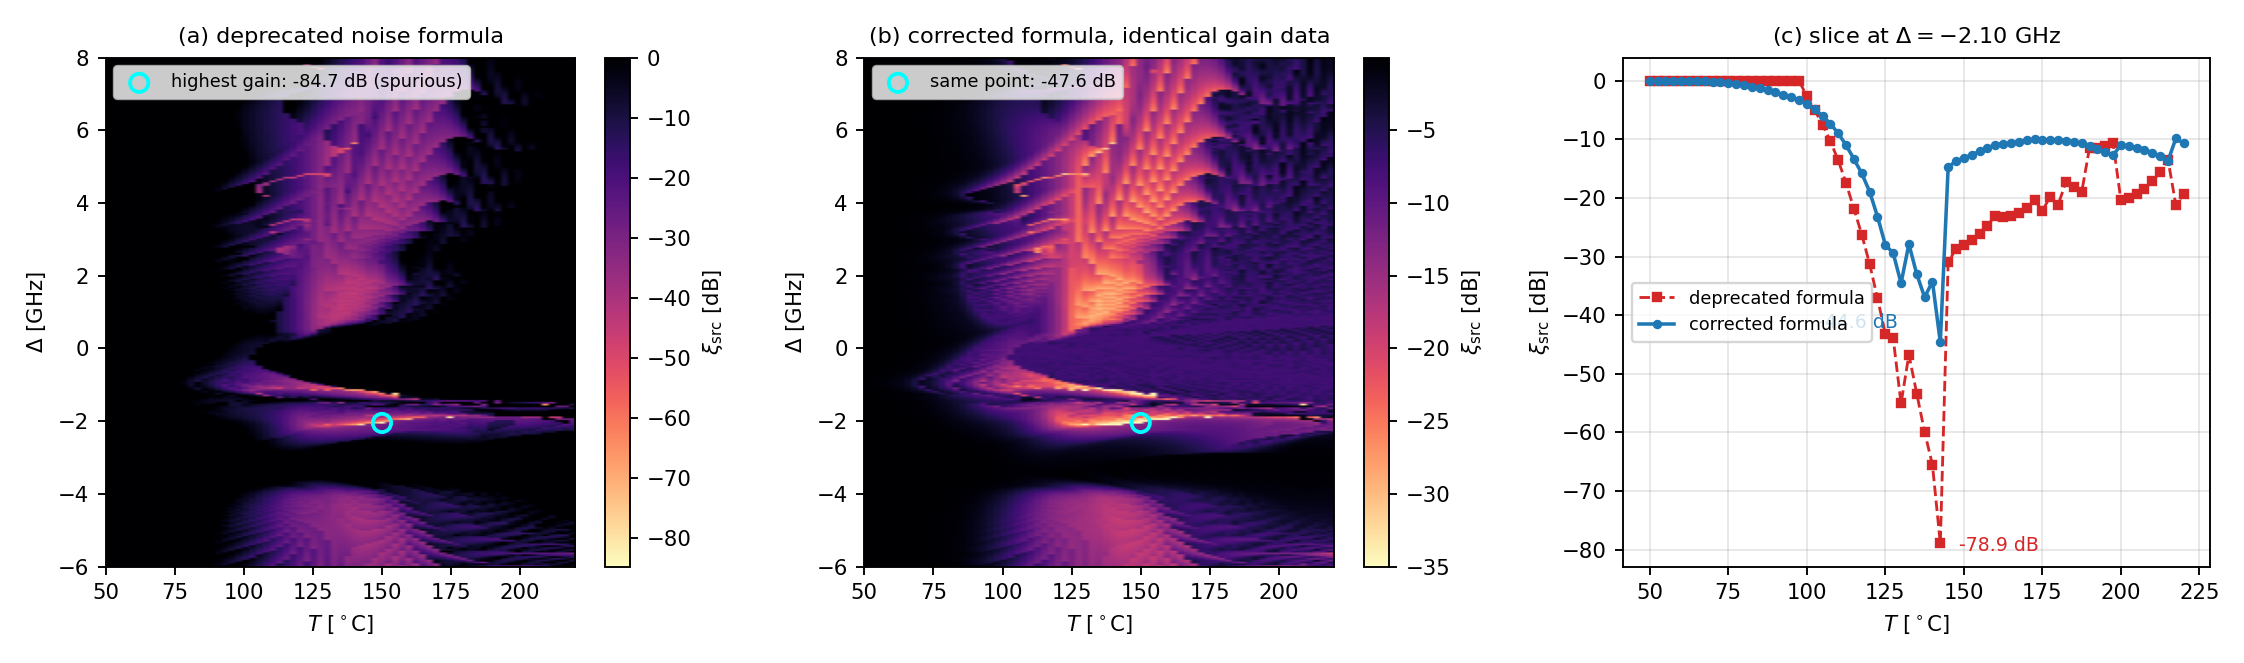
\includegraphics[width=\textwidth]{fig4_formula_bug.png}
\caption{The Stage-III formula bug, demonstrated on identical archived gain
data from the wide ideal-detection scan (source term only; in-cell loss
factored out). (a)~The deprecated formula, Eq.~\eqref{eq:oldformula},
produces a spurious ultra-deep region; at the archive's highest-gain point
(circle) it yields $-84.7\dB$, reproducing the magnitude of the originally
reported $-82.0\dB$ optimum. (b)~The corrected formula,
Eq.~\eqref{eq:sideal}, evaluated on the very same $(G_s,G_c)$ pairs.
(c)~Slice at $\Delta=-2.10\GHz$: the two formulas diverge exactly where the
gain grows, by $\sim 34\dB$ at $T=142.5\degC$.}
\label{fig:formulabug}
\end{figure}

\subsection{Collateral hardening: the gain-gap consistency gate}
The corrected formula introduced a new failure mode of its own. Since
$S_{\mathrm{src}}\propto(G_s-G_c)^2$, any point where the two gains happen
to be \emph{equal} reports perfect squeezing --- even in background regions
with no parametric interaction at all, where $G_s\approx G_c\approx 1$.
Physically, lossless seeded parametric gain enforces $G_s-G_c=1$; departures
signal either absorption or a numerically untrustworthy point. All scans
from this stage onward therefore apply a \textbf{twin-beam gain-gap
consistency criterion}: a point is trusted only if
\begin{equation}
0.5 \;\le\; G_s-G_c \;\le\; 1.5 ,
\label{eq:gapgate}
\end{equation}
and $\delta$-optimization is restricted to trusted candidates. At the
reference operating point the gap stays within $[0.55,0.98]$ across the
full $\delta$ scan, comfortably inside the gate.

At the same stage, the collisional decoherence channels of
Sec.~\ref{sec:model} were added to the model. With them, the
finite-detection squeezing acquires a temperature optimum near
$T\sim 120$--$135\degC$ and degrades at higher temperature --- the first time the simulation
reproduced the experimentally familiar high-temperature rollover rather than
saturating at the floor indefinitely.

The general lesson of Stage III is transferable: when a physics formula is
corrected, every downstream consumer must be re-verified, and an incorrect
formula may have been silently \emph{masking} out-of-domain evaluations that
the corrected formula then exposes (here, the $G_s=G_c$ background points
that necessitated the gate of Eq.~\eqref{eq:gapgate}).

%==================================================================
\section{Stage IV: gain without cost --- the missing absorption channels}
\label{sec:stage4}
%==================================================================

\subsection{An internally contradictory optimum}
After the formula correction, the finite-detection scans still placed the
global optimum at $\Delta=-2.20\GHz$, $T=135\degC$ with a probe gain of
$G_s=636$ --- while simultaneously reporting an in-cell optical depth of
essentially zero at that point. That combination is self-contradictory: a
parametric gain of several hundred requires a strong near-resonant atomic
response, and a strong response absorbs. The contradiction arose because the
objective function was blind to two costs. First, the noise formula
Eq.~\eqref{eq:sideal} depends only on the gain \emph{difference}: with
$G_s-G_c\approx 1$, a point with $G_s=636$ scores as well as one with
$G_s=27$, even though nothing in the model charged for the absorption that
generated the factor-600 gain. Second, only the \emph{probe} arm's
absorption was being applied: at far-red detunings the probe sits several
GHz from resonance and is indeed transparent, but the \emph{conjugate}
(at $f_c=2\Delta-f_{\mathrm{probe}}$) then lands near the $F{=}2\to F'$
manifold and is strongly absorbed --- at zero model cost.

\subsection{The extended excess-noise model}
Stage IV closed both holes (Sec.~\ref{sec:noisemodel}): each sideband is
attenuated by the validated linear absorption at its \emph{own} optical
frequency (no adjustable parameter), unequal arm losses enter through the
balanced-detector noise model, and pump scatter anchored to the pump optical
depth is added with the single residual coefficient $\kappa$. The effect on
the artifact was decisive: the former optimum at $(-2.20\GHz, 135\degC)$,
where the conjugate-arm optical depth is in fact $0.22$, dropped from
$-8.83$ to $-5.41\dB$, and the global optimum moved to a moderate-gain
point ($G_s=27$ as computed at this stage). Removing the detection floor
($\eta=1$) confirmed that the change is source physics rather than a
detection effect (Fig.~\ref{fig:excessnoise}): without the excess-noise
channels the ideal scan ran away to $-36.6\dB$ at the $G_s=636$ coordinate,
while the extended model capped the ideal optimum at $-15.5\dB$ at the same
moderate-gain location as the finite-detection optimum.

\begin{figure}[ht]
\centering
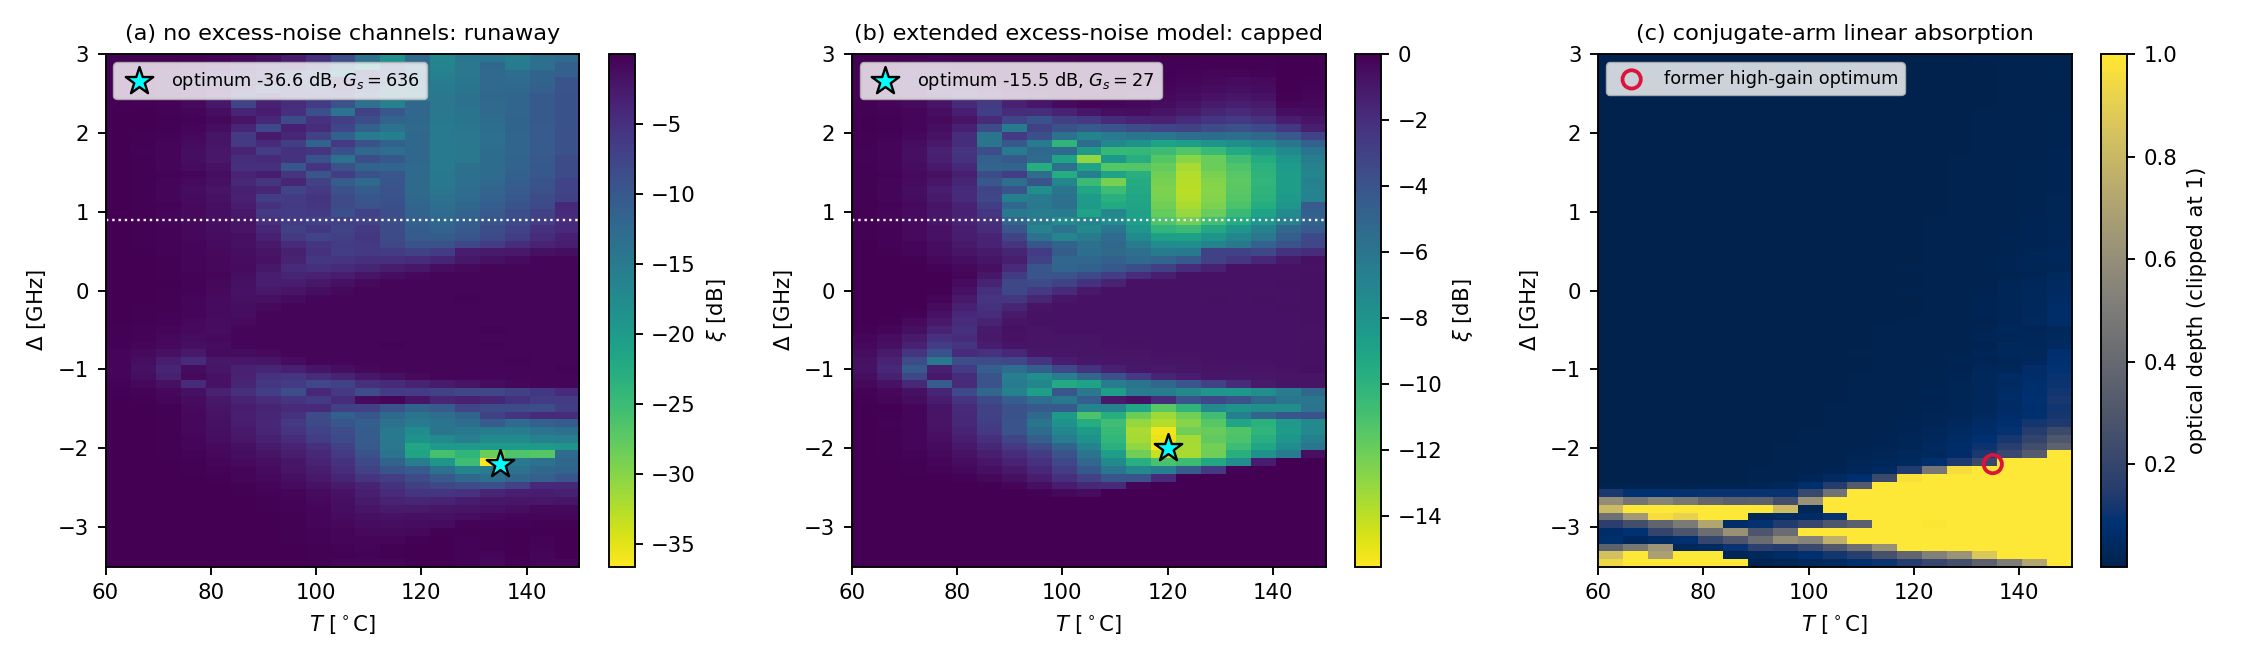
\includegraphics[width=\textwidth]{fig5_excess_noise.png}
\caption{Stage-IV hardening, shown at ideal detection ($\eta=1$) where the
contrast is not compressed by the detection floor (all panels use
Stage-IV-era scans, i.e.\ the sideband-beat sign error corrected in Stage V
is still present, so the coordinates are historical). (a)~Without the
excess-noise channels the ideal optimum (star) runs away to $-36.6\dB$ at
an extreme gain, $G_s=636$, at a nominally transparent point.
(b)~With per-sideband absorption and pump scatter charged, the ideal
optimum is capped at $-15.5\dB$ at a moderate gain, $G_s=27$. (c)~The
mechanism: the conjugate-arm linear optical depth is large exactly where
the uncharged model had found free gain (circle marks the former optimum).
The dotted horizontal line marks the reference experiment's detuning
$+0.9\GHz$.}
\label{fig:excessnoise}
\end{figure}

\subsection{An honest near-degeneracy}
With the artifact removed, a physical question remained: the optimum stayed
at \emph{red} pump detuning ($\Delta\approx-2\GHz$ as computed at this
stage), whereas the experimental literature operates at
$\Delta\approx+0.8$--$1.0\GHz$ \cite{McCormick2007,Pooser2009,Sim2025}.
The red-side preference is not a numerical accident. At
$\Delta\approx-2\GHz$ the pump sits about $1\GHz$ to the blue of the
$F{=}3\to F'{=}3$ manifold --- the mirror image of the conventional
operating point, but anchored on the \emph{more populated} $F=3$ ground
state ($7/12$ of the population versus $5/12$ in $F=2$), and with the seeded
probe pushed to a spectrally clean far-red position where its absorption is
small. Both effects are real physics. However, the model is a steady-state
description with a fixed ground-state population distribution: it does not
include the optical pumping by which a pump parked near the $F=3$ manifold
would deplete $F=3$ itself. That depletion is precisely what should erode
the red-side advantage in a real experiment. The two lobes are, moreover,
nearly degenerate --- $0.28\dB$ apart at this stage, $0.32\dB$ in the final
model. We therefore report the red/blue asymmetry as a model-level
near-degeneracy, not as a firm experimental prediction; resolving it
requires optical-pumping dynamics beyond the present model.

%==================================================================
\section{Stage V: the beat-sign audit and the final operating point}
\label{sec:stage5}
%==================================================================

\subsection{The last defect: a sign error in the sideband beat}
The Floquet solver takes as input the beat frequency between the pump and
the seeded sideband. With the scan coordinate defined by
Eq.~\eqref{eq:tpd}, the physical beat is
$|\omega_{\mathrm{pump}}-\omega_{\mathrm{seed}}| = \nu_{\mathrm{HF}}-\delta$
on the $(-)$ branch. An audit of the solver input revealed that all previous
stages had used $\nu_{\mathrm{HF}}+\delta$ --- the wrong sign of $\delta$ for
the standard seeded readout. Because $|\delta|$ is small
($\lesssim 0.5\GHz$) compared with $\nu_{\mathrm{HF}}$, the error had
distorted rather than destroyed the landscape, which is why it survived
four stages of scrutiny; it was caught only by writing the beat relation
down symbolically and checking the code paths against it. After the
correction (applied identically in both numerical code paths) the full
regression baseline of the simulation was re-anchored, and every scan below
was recomputed from scratch.

\subsection{The final finite-detection frontier}
Figure~\ref{fig:finalfrontier} and Table~\ref{tab:final} give the corrected
finite-detection landscape at the reference efficiency $\eta=0.8694$
($\Delta\in[-3.5,+3.0]\GHz$, $T\in[60,150]\degC$, $\delta$ optimized within
the trust gate at each point). The global optimum moves from the Stage-IV
coordinate to
\begin{equation}
\boxed{\;\Delta=-1.50\GHz,\quad T=110\degC,\quad \delta=-280\MHz:\quad
\xi=-8.10\dB,\ G_s=22.6\; }
\end{equation}
with a healthy gain gap $G_s-G_c=0.62$ and a small probe optical depth
($\approx 0.02$). The former Stage-IV optimum at $(-2.0\GHz,120\degC)$,
re-evaluated with the corrected beat, is no longer optimal ($-7.00\dB$,
$G_s=7$). The best blue-side operating point is $+1.40\GHz$, $125\degC$ with
$-7.78\dB$ --- $0.32\dB$ shallower than the red-side optimum, preserving the
near-degeneracy discussed in Sec.~\ref{sec:stage4}. A fixed readout at the
reference experiment's nominal point ($+0.90\GHz$, $121\degC$,
$\delta=-8\MHz$) gives $-7.20\dB$, to be compared with the measured
$-7.8\dB$ and gain $\approx 15$ of Ref.~\cite{Sim2025} (simulated
$G_s=14.0$): the simulation reproduces the measured squeezing scale, gain
scale, and temperature scale at the experiment's own operating point.

\begin{table}[ht]
\centering
\caption{Final (Stage-V) finite-detection results at $\eta=0.8694$. The
reference-experiment row is a fixed readout at the nominal coordinates of
Ref.~\cite{Sim2025}; all other rows optimize $\delta$ within the trust gate.}
\label{tab:final}
\small
\begin{tabular}{lrrrrrr}
\toprule
Point & $\Delta$ [GHz] & $T$ [$^\circ$C] & $\delta$ [MHz] & $\xi$ [dB] &
$G_s$ & $G_s-G_c$\\
\midrule
Global optimum & $-1.50$ & $110$ & $-280$ & $-8.10$ & $22.6$ & $0.62$\\
Best blue-side lobe & $+1.40$ & $125$ & $0$ & $-7.78$ & $39.0$ & $0.70$\\
Reference-experiment readout & $+0.90$ & $121$ & $-8$ & $-7.20$ & $14.0$ & $0.90$\\
Stage-IV optimum, re-evaluated & $-2.00$ & $120$ & $-280$ & $-7.00$ & $7.0$ & $0.85$\\
\bottomrule
\end{tabular}
\end{table}

\begin{figure}[ht]
\centering
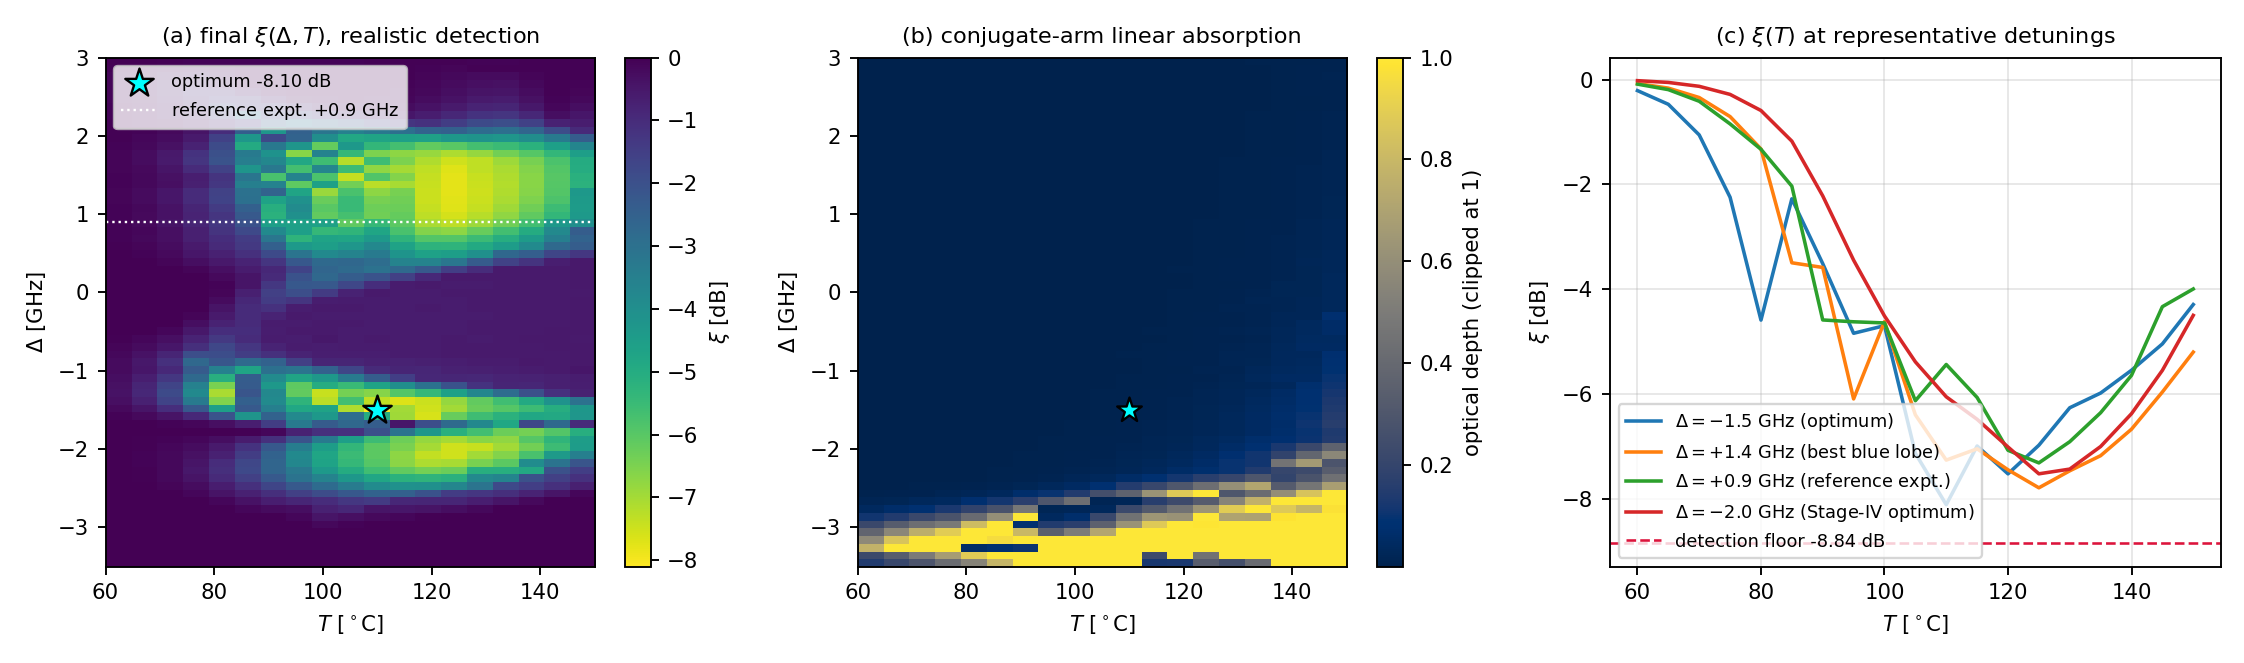
\includegraphics[width=\textwidth]{fig6_final_frontier.png}
\caption{Final finite-detection landscape ($\eta=0.8694$, floor
$-8.84\dB$). (a)~$\xi(\Delta,T)$ with the global optimum (star) at
$(-1.50\GHz,110\degC)$ and the reference experiment's detuning (dotted).
(b)~Conjugate-arm linear optical depth: the excess-noise channel that
suppresses the far-red high-gain region. (c)~$\xi(T)$ at representative
detunings; the red- and blue-side lobes are nearly degenerate, and no curve
crosses the detection floor (dashed). The visible jaggedness of the slices
reflects the $17.5\MHz$ $\delta$-grid of the survey scan; the tolerance
analysis of Sec.~\ref{sec:tolerance} uses a $5\MHz$ grid.}
\label{fig:finalfrontier}
\end{figure}

\subsection{Ideal-detection source limit}
Re-reading the same scan at $\eta=1$ (Fig.~\ref{fig:ideallimit}) removes
the detection floor without moving the optimum: the deepest ideal-detection
squeezing is $-15.62\dB$ at exactly the same $(\Delta,T,\delta)$ as the
finite-detection optimum. The floor thus only compresses the landscape; the
\emph{location} of the optimum is set by in-cell absorption, i.e.\ it is
source physics. The contrast with the cost-blind objective remains stark
even after the beat correction: without the excess-noise channels the ideal
scan runs away to $-34.9\dB$ at a $G_s\approx 1400$ coordinate that the full
model evaluates at just $-3.9\dB$. On the blue side the ideal-detection
lobe is $-13.9\dB$, $1.7\dB$ shallower than the red-side optimum --- the
near-degeneracy widens when the floor no longer compresses both lobes.

\begin{figure}[ht]
\centering
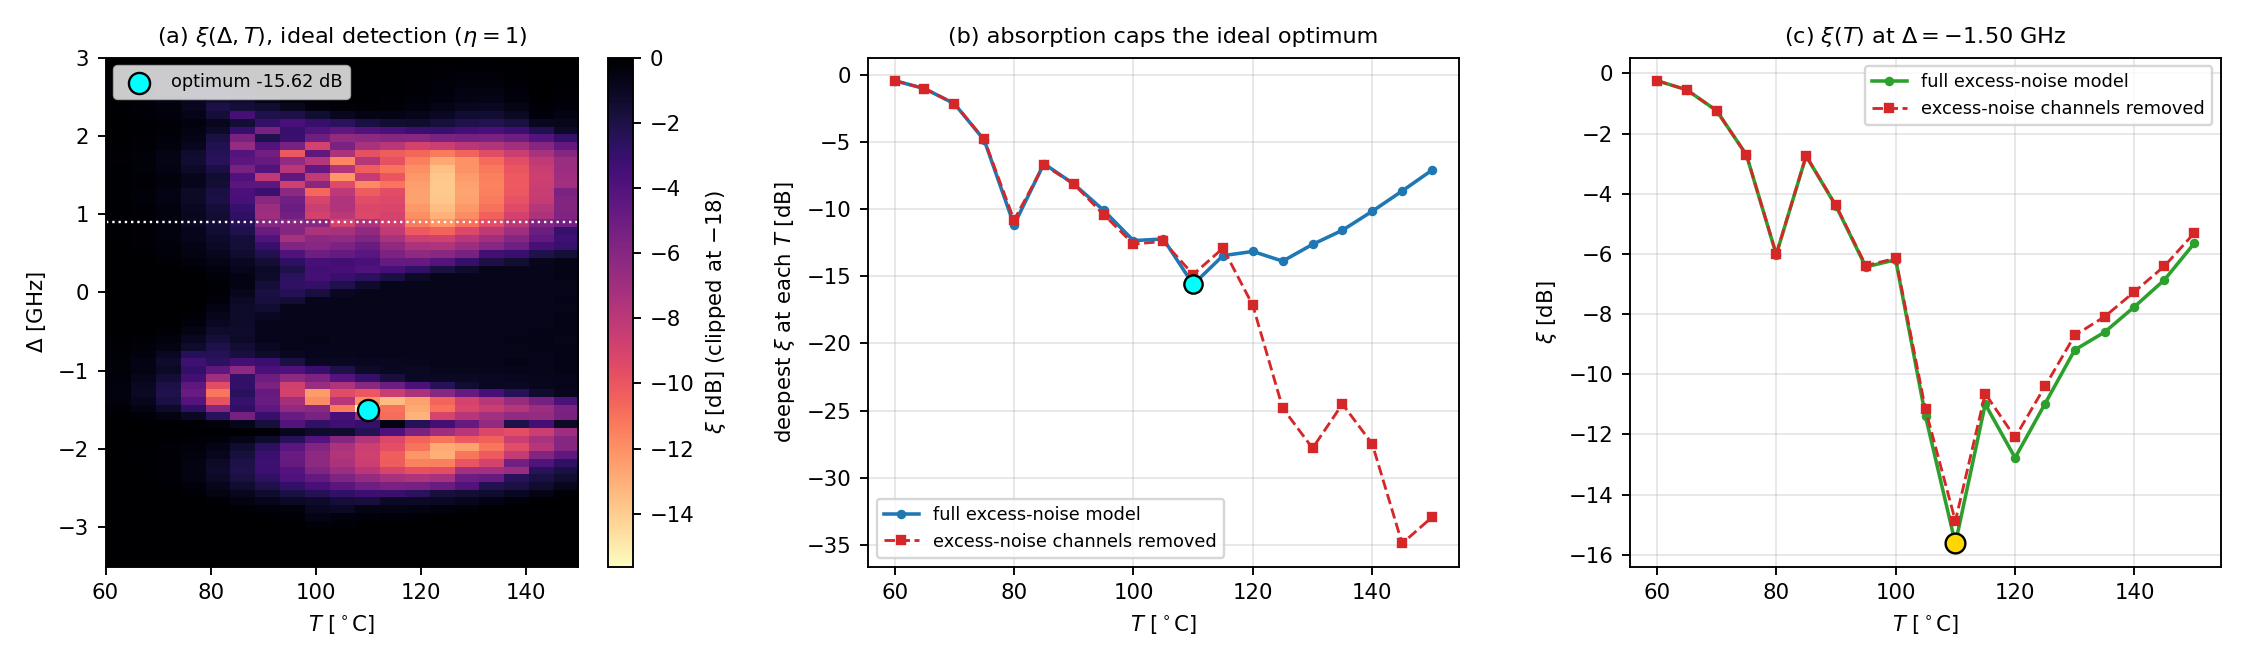
\includegraphics[width=\textwidth]{fig7_ideal_limit.png}
\caption{Ideal-detection ($\eta=1$) source limit of the final model.
(a)~$\xi(\Delta,T)$; the optimum (circle) coincides in position with the
finite-detection optimum of Fig.~\ref{fig:finalfrontier}. (b)~Deepest
trusted squeezing at each temperature: with the excess-noise channels the
optimum is capped at $-15.6\dB$ near $110\degC$ (circle), whereas the
cost-blind objective (dashed) runs away toward ever deeper values at high
temperature. (c)~The same comparison along the optimal-detuning slice.}
\label{fig:ideallimit}
\end{figure}

\subsection{Two-photon detuning and beam-angle geometry}
The survey scans treat $\delta$ as an internal optimization variable on a
coarse grid and pin the pump--probe angle at the experimental
$0.32^{\circ}$. A dedicated four-dimensional scan around the ideal-detection
optimum ($\Delta\in[-1.56,-1.44]\GHz$, $T\in[96,114]\degC$,
$\theta\in[0,0.36]^{\circ}$, $\delta\in[-420,-160]\MHz$, trust gate applied
throughout) treats both explicitly (Fig.~\ref{fig:geometry}). At the default
geometry the detailed scan finds its best trusted point at $-14.8\dB$
($\Delta=-1.54\GHz$, $T=106\degC$, $\delta=-287\MHz$), compared with
$-15.6\dB$ on the coarse survey grid (the two scans differ in $\delta$
resolution and scan volume); in round numbers, the source limit of the
default $0.32^{\circ}$ geometry is $-15\dB$.
Relaxing the angle opens a distinct \emph{low-angle ridge}: as
$\theta\to 0$ the longitudinal phase mismatch and the Gaussian-overlap
penalty relax together, the optimal temperature falls, and the deepest
trusted point reaches $-20.7\dB$ at $\theta=0.02^{\circ}$
($\Delta=-1.66\GHz$, $T=102\degC$, $\delta=-307\MHz$). We deliberately
report the ridge as a \emph{geometry-conditional diagnostic}, not as a
replacement optimum: in a real seeded FWM setup the crossing angle is tied
to beam separation, spatial filtering, and pump-leakage rejection, and the
pump-scatter coefficient of the model has not been recalibrated for
near-collinear geometry. (The unconstrained scan also finds nominally deeper
raw points, e.g.\ $-27.6\dB$, but they fail the gain-gap gate,
$G_s-G_c\approx 0$, and are rejected --- the Stage-III guardrail doing its
job.)

\begin{figure}[ht]
\centering
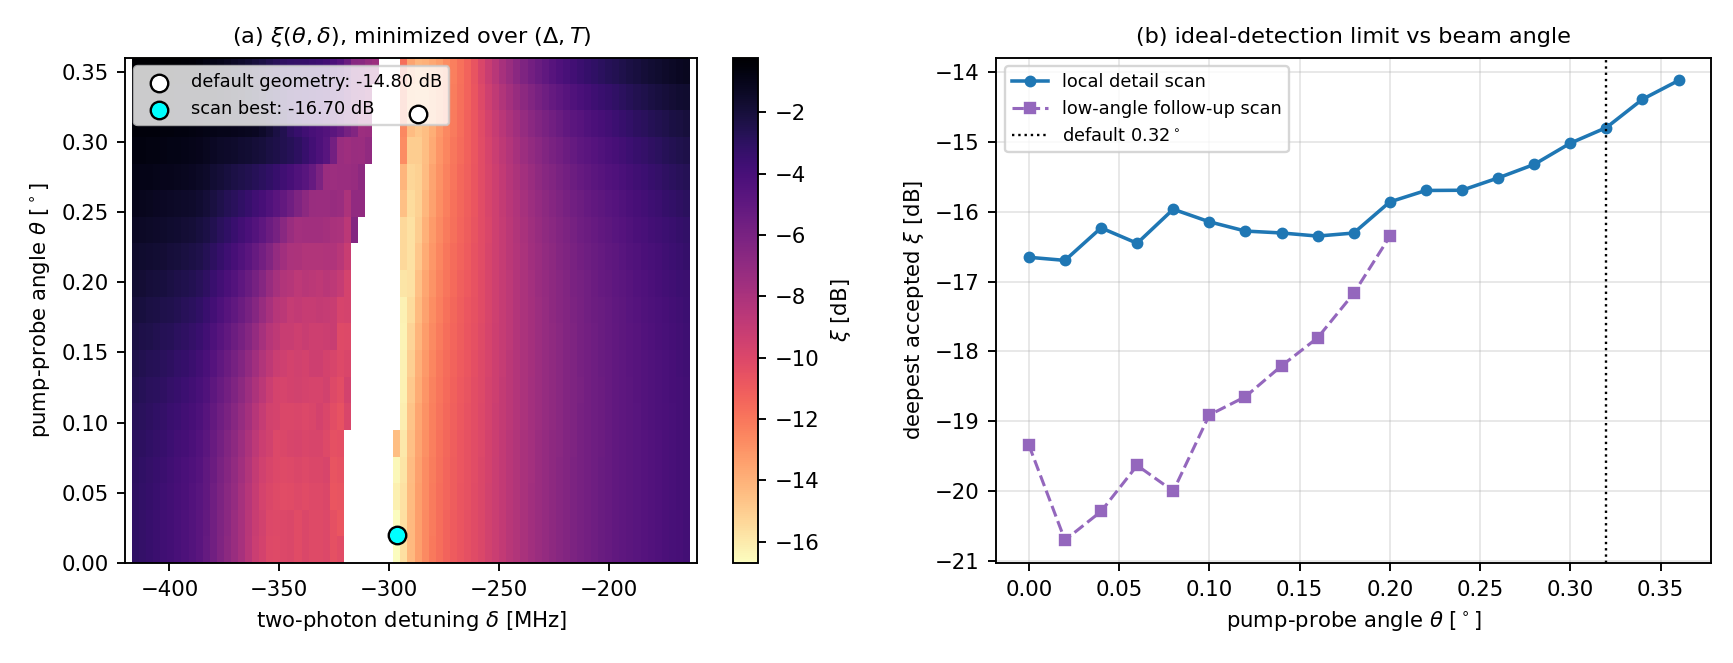
\includegraphics[width=0.92\textwidth]{fig8_geometry.png}
\caption{Geometry study at ideal detection (trust gate applied; blank
columns in (a) contain no trusted points --- there the gain gap collapses
and the noise formula is not meaningful, cf.\ Eq.~\eqref{eq:gapgate}).
(a)~$\xi(\theta,\delta)$ minimized over the local $(\Delta,T)$ block; the
white marker is the best point at the default $0.32^{\circ}$ geometry, the
cyan marker the best trusted point of the block. (b)~Deepest trusted
squeezing versus crossing angle, from the local detail scan and from a
dedicated low-angle follow-up scan: the low-angle ridge reaches $-20.7\dB$
at $\theta=0.02^{\circ}$ but is tied to geometry calibration outside the
model's validated range.}
\label{fig:geometry}
\end{figure}

%==================================================================
\section{Tolerance of the recommended operating point}
\label{sec:tolerance}
%==================================================================
For experimental use, the location of the optimum matters less than how fast
the squeezing degrades when a knob drifts. We therefore performed
one-dimensional tolerance scans of the five experimentally accessible
variables around the final optimum
$(\Delta,T,\delta)=(-1.50\GHz,110\degC,-280\MHz)$, with everything else
pinned (Fig.~\ref{fig:tolerance}, Table~\ref{tab:tolerance}). Each
recomputed scan is read out in two ways: \textbf{fixed $\delta$}, modeling
pure drift in the common configuration where the probe is derived from the
pump by a fixed RF offset; and \textbf{re-optimized $\delta$}, modeling an
experimenter who rescans the two-photon detuning after the drift. The
detection-loss axis is an analytic remap of the stored gains
(Sec.~\ref{sec:noisemodel}), verified to reproduce the solved value at the
reference loss to machine precision. Degradation thresholds of $+0.25$,
$+0.5$, and $+1.0\dB$ correspond to $+5.9\%$, $+12.2\%$, and $+25.9\%$ in
linear noise power; the discussion below uses $+0.5\dB$ as the
representative budget.

One technical caveat uncovered here feeds back into the survey scans: the
$17.5\MHz$ $\delta$-grid used in the wide scans can miss the narrow trusted
minimum near a gate boundary and make a best-$\delta$ readout look worse
than it is. The tolerance scans therefore use a $5\MHz$ grid; the optimum
quoted in Sec.~\ref{sec:stage5} is stable against this refinement.

\begin{table}[ht]
\centering
\caption{Tolerance windows around the recommended operating point
(fixed-$\delta$ readout; drift measured from the optimum). The bracketed
entries give the $+0.5\dB$ window when $\delta$ is re-optimized after the
drift.}
\label{tab:tolerance}
\small
\begin{tabularx}{\textwidth}{llll>{\raggedright\arraybackslash}X}
\toprule
Variable & $+0.25\dB$ & $+0.5\dB$ & $+1.0\dB$ & Remark\\
\midrule
$\Delta$ [MHz] & $-16/{+}130$ & $-32/{+}155$ & $-55/{+}185$ &
blue side enters the gap-collapse region; re-optimizing $\delta$ widens the
$+0.5\dB$ window to $[-75/{+}158]$ and, jointly with $\delta$, to the
$\pm0.1\GHz$ scale\\
$\delta$ [MHz] & $-8.0/{+}2.1$ & $-9.6/{+}4.2$ & $-10.4/{+}7.3$ &
narrowest absolute window; steep cliff on the blue side, spurious
gate-failing dip near $-307\MHz$ on the red side\\
$T$ [$^\circ$C] & $-2.2/{+}9.5$ & $-3.3/{+}12.0$ & $-5.0/{+}18.1$ &
cliff on the cold side; the 1-D slice minimum sits near $112\degC$
($-8.17\dB$), so running $1$--$2\degC$ hot is the safe bias\\
Seed power & \multicolumn{3}{l}{$1$--$64\,\mu$W: no change ($<0.004\dB$)} &
model contains no seed-power-dependent technical noise; avoid detector
saturation\\
Loss [\%-points] & $+1.0$ & $+2.1$ & $+4.5$ &
slope $\simeq 0.22\dB$ per \%-point; eliminating the reference $5.5\%$ loss
would deepen the optimum to $-9.77\dB$ ($1.67\dB$ gain)\\
\bottomrule
\end{tabularx}
\end{table}

\begin{figure}[ht]
\centering
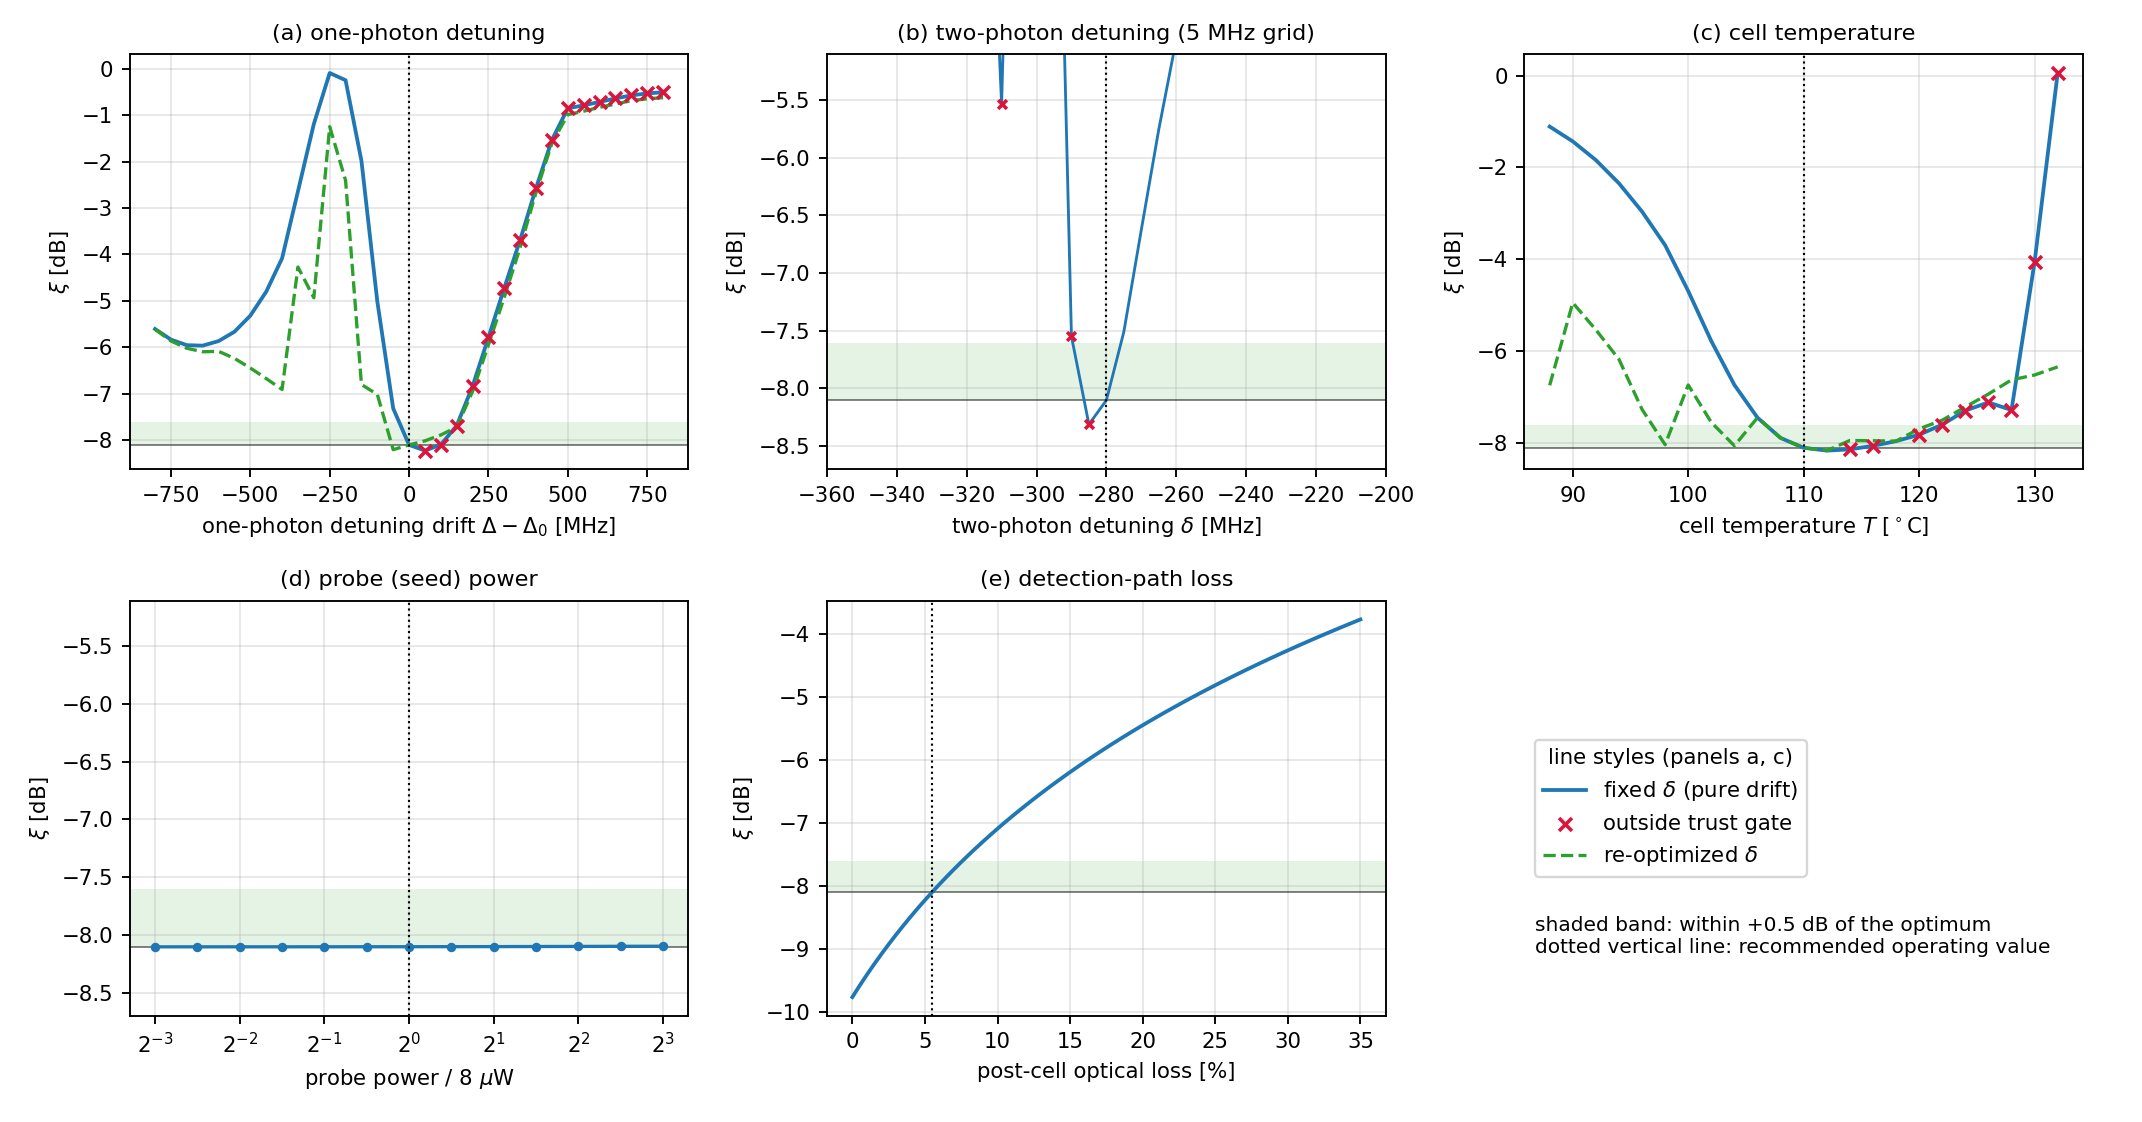
\includegraphics[width=\textwidth]{fig9_tolerance.png}
\caption{One-dimensional tolerance scans around the recommended operating
point ($\eta=0.8694$). Solid: fixed $\delta$ (pure drift); dashed:
$\delta$ re-optimized within the trust gate; crosses: fixed-$\delta$ points
that leave the trust gate (their apparent depth is not to be believed ---
notably the seemingly favorable blue-side excursions in (a) and the dip
near $\delta=-307\MHz$ in (b)). The shaded band is the $+0.5\dB$ budget.}
\label{fig:tolerance}
\end{figure}

The practical checklist, in the order a lab should work through it when the
squeezing is shallower than expected:
\begin{enumerate}[nosep]
\item \textbf{Detection loss.} The only variable that moves the attainable
      floor itself: $0.22\dB$ is lost per percentage point, uniformly and
      irrecoverably. Check window transmissions, detector quantum
      efficiency, mode matching, and clipping first --- and note that loss
      improvement is also the largest available upgrade ($1.67\dB$ from
      removing the reference $5.5\%$).
\item \textbf{Two-photon detuning $\delta$.} The narrowest window
      ($-9.6/{+}4.2\MHz$ at $+0.5\dB$) with a cliff on the blue side ---
      but it is set by RF electronics, so genuine drift is unlikely; the
      real risk is targeting the wrong value. It is also the cheapest knob
      to verify (an RF rescan), so rescan $\delta$ immediately after
      checking loss. Do not let an optimizer walk into the seemingly deep
      dip near $-307\MHz$: it fails the gain-gap gate and is an artifact.
\item \textbf{One-photon detuning $\Delta$.} The effective red-side window
      is about $32\MHz$; apparently favorable blue-side
      values sit in the gap-collapse region and should not be trusted. A
      pump lock at the $10\MHz$ level is appropriate. Because $\Delta$ and
      $\delta$ are strongly coupled, always rescan $\delta$ after moving
      $\Delta$ --- jointly they tolerate an order of magnitude more drift.
\item \textbf{Temperature.} Asymmetrically forgiving
      ($-3.3/{+}12\degC$); controller stability is a non-issue and the
      practical risk is absolute calibration (sensor offset). Bias
      $1$--$2\degC$ hot, away from the cold-side cliff.
\item \textbf{Seed power.} Insensitive across $1$--$64\,\mu$W in the model
      (the susceptibilities are seed-independent and pump depletion is
      negligible at these powers); experimentally, only detector saturation
      matters. Check last.
\end{enumerate}

%==================================================================
\section{Discussion}
\label{sec:discussion}
%==================================================================

\subsection{What limits the squeezing --- and what does not}
Across all five stages one hierarchy has remained stable. The \emph{depth} of
the observable squeezing is set almost entirely by the detection efficiency:
once $G_s\gtrsim 30$, additional gain buys nothing
(Fig.~\ref{fig:floor}), while every percentage point of detection loss
costs $\approx 0.2\dB$ irrecoverably. The \emph{location} of the optimum,
by contrast, is set by in-cell absorption --- the competition between
parametric gain and the linear optical depths of \emph{both} sidebands ---
as demonstrated by the fact that removing the detection floor entirely does
not move the optimum (Sec.~\ref{sec:stage5}). Finally, loss of any kind can
only push the intensity-difference noise toward shot noise, never above it
(Eq.~\eqref{eq:eta}); measured anti-squeezing is always excess noise, with
the leakage of the gain-amplified intensity-sum noise through detector or
loss imbalance the most dangerous channel at high gain. This is one more
reason the efficient-frontier philosophy --- reach the floor at the lowest
temperature, gain, and optical depth --- is also the robust experimental
choice.

\subsection{A guardrail checklist for simulation-based squeezing predictions}
Each of the defects in this study was caught not by comparison with
experiment but by an internal-consistency check. We collect them here as a
checklist for similar simulation efforts:
\begin{enumerate}[nosep]
\item \textbf{Detection-floor bound.} At detection efficiency $\eta$, no
      point may be deeper than $10\log_{10}(1-\eta)$
      (Eq.~\eqref{eq:floor}). This holds regardless of the source model;
      treat any violation as a numerical error, and treat a large
      \emph{plateau at} the floor as a sign that the optimization question
      itself is degenerate (Stage I).
\item \textbf{Conserved-quantity consistency gate.} Enforce the physical
      constraint of the process --- here $G_s-G_c=1$ for lossless seeded
      parametric gain, gated as Eq.~\eqref{eq:gapgate} --- and exclude
      untrusted points from optimization. A formula that is exact on the
      constraint manifold can be spectacularly wrong off it (Stages III and
      V: background points and raw low-angle optima reporting spurious
      perfect squeezing).
\item \textbf{Formula cross-check on identical data.} When two expressions
      for the same observable exist, evaluate both on the same stored
      intermediate data. A divergence that \emph{grows with gain} indicates
      a wrong asymptote; sensitivity to floating-point cancellation
      indicates an expression that must be reformulated in terms of small
      differences (Stage III).
\item \textbf{Cost-charging test.} Ask whether the optimum survives when
      the physical costs of its own figure of merit are charged. An optimum
      whose reported diagnostics are internally contradictory --- here,
      $G_s=636$ with zero reported absorption --- is an artifact of an
      objective blind to a channel (Stage IV).
\item \textbf{Sign and convention audit.} Write the frequency/sign
      relations down symbolically and verify every code path against them;
      small-parameter sign errors distort rather than destroy the landscape
      and can survive long scrutiny (Stage V). Re-anchor all regression
      baselines after each physics fix.
\item \textbf{Resolution audit at gate boundaries.} A coarse grid in the
      optimized variable can interact with a trust gate to misreport the
      best trusted value (the $17.5\MHz$ versus $5\MHz$ $\delta$-grid in
      Sec.~\ref{sec:tolerance}).
\end{enumerate}

\subsection{Limitations}
The model is a steady-state description with a fixed thermal ground-state
population; it does not include optical pumping, which is the missing
physics most likely to decide the red/blue near-degeneracy of
Sec.~\ref{sec:stage4} in favor of the conventional blue-side operating
point. The pump-scatter coefficient is calibrated only at the reference
geometry, so the low-angle ridge of Sec.~\ref{sec:stage5} is a design
target, not a prediction. Seed-power-dependent technical noise (detector
saturation, laser intensity noise) is outside the model, as are all
excess-noise channels beyond per-sideband absorption and pump scatter; the
quoted depths are therefore best-case values for the
efficiency-and-absorption budget alone, not guaranteed measurement
outcomes. Finally, the corrected noise
formula is itself limited by double-precision arithmetic above
$G\sim 10^{7}$, far outside the recommended operating regime.

%==================================================================
\section{Conclusion}
%==================================================================
A first-principles steady-state simulation of double-$\Lambda$ four-wave
mixing on the \Rb{} D1 line, calibrated once against the reference
experiment of Ref.~\cite{Sim2025}, predicts a recommended operating point at
$\Delta=-1.50\GHz$, $T=110\degC$, $\delta=-280\MHz$ with
$\xi=-8.10\dB$ at $\eta=0.8694$ --- within $0.7\dB$ of the detection floor
at a moderate gain of $G_s\approx 23$ --- and reproduces the measured
squeezing, gain, and temperature scales of the reference experiment at its
own operating point. The tolerance budget around the recommended point is
dominated by detection loss ($0.22\dB$ per percentage point) and by the
two-photon detuning ($-9.6/{+}4.2\MHz$ for $+0.5\dB$), with temperature
asymmetrically forgiving and seed power irrelevant; when squeezing is lost,
the efficient checking order is loss, then a $\delta$ rescan, then the pump
lock, then temperature calibration, then seed power. At ideal detection the
same operating point reaches $-15.6\dB$, and a near-collinear geometry
could in principle reach $-20.7\dB$, though the latter requires geometry
calibration beyond the model's validated range. The red-side optimum is
nearly degenerate with the conventional blue-side operating point
($0.32\dB$), and deciding between them requires optical-pumping physics
absent from the present model.

Equally important are the negative results: a $-82\dB$ ``theoretical
optimum'' that was the artifact of a catastrophically canceling formula, an
extreme-gain optimum produced by an objective function that failed to charge
for absorption, and a sign error that survived four model revisions. All were caught by cheap
internal-consistency guardrails --- a detection-floor bound, a
conserved-quantity gate, formula cross-evaluation on identical data, and a
symbolic sign audit --- that we recommend as standard practice for any
simulation used to steer a squeezing experiment.

%==================================================================
\section*{Data availability}
%==================================================================
The complete simulation source code, the archived scan data underlying every
figure, the figure-generation scripts, and the regression tests that pin the
calibrated reference behavior are openly available in the GitHub repository
of Ref.~\cite{repo}. The historical scans of Stages I--II are shown in
their archived rendered form (Figs.~\ref{fig:stage1plateau} and
\ref{fig:stage2od}), as their raw grids were later overwritten; all other
figures are regenerated directly from the archived raw data.

%==================================================================
\begin{thebibliography}{9}
%==================================================================
\bibitem{McCormick2007}
C.~F. McCormick, V.~Boyer, E.~Arimondo, and P.~D. Lett,
``Strong relative intensity squeezing by four-wave mixing in rubidium
vapor,'' Opt.\ Lett.\ \textbf{32}, 178--180 (2007).

\bibitem{Pooser2009}
R.~C. Pooser, A.~M. Marino, V.~Boyer, K.~M. Jones, and P.~D. Lett,
``Quantum correlated light beams from non-degenerate four-wave mixing in an
atomic vapor: the D1 and D2 lines of $^{85}$Rb and $^{87}$Rb,''
Opt.\ Express \textbf{17}, 16722--16730 (2009).

\bibitem{Jasperse2011}
M.~Jasperse, L.~D. Turner, and R.~E. Scholten,
``Relative intensity squeezing by four-wave mixing with loss: an analytic
model and experimental diagnostic,''
Opt.\ Express \textbf{19}, 3765--3774 (2011).

\bibitem{Sim2025}
G.~Sim, H.~Kim, and H.~S. Moon,
``Intensity-difference squeezing from four-wave mixing in hot $^{85}$Rb and
$^{87}$Rb atoms in single diode laser pumping system,''
Sci.\ Rep.\ \textbf{15}, 7727 (2025).

\bibitem{Allen2026}
C.~H. Allen, M.~San Soucie, R.~J. Benson, O.-M. Glezakou-Elbert,
R.~Jimenez, J.~Morrell-Falvey, and Y.-Z. Ma,
``Long-term stabilization of intensity-difference squeezing from four-wave
mixing in rubidium vapor,''
Opt.\ Express \textbf{34}, 19382--19399 (2026).

\bibitem{repo}
S.~Park, \emph{FWM squeezing simulation --- source code, scan archives, and
figure scripts}, GitHub repository,
\url{https://github.com/Shake2313/fwm-squeezing-app} (2026).

\end{thebibliography}

\end{document}
